% !TeX program = pdflatex
% Compilar desde la raíz: latexmk -cd -pdf informe/Ficha_Proyecto_EN.tex
\documentclass[10pt,a4paper]{article}
\usepackage[margin=16mm,top=19mm,bottom=17mm,headheight=24pt]{geometry}
\usepackage{iftex}
\ifPDFTeX
  \usepackage[T1]{fontenc}
  \usepackage[utf8]{inputenc}
  \usepackage{lmodern}
  \renewcommand{\familydefault}{\sfdefault}
\else
  \usepackage{fontspec}
  \IfFontExistsTF{DejaVu Sans}{\setmainfont{DejaVu Sans}\setsansfont{DejaVu Sans}}{\setmainfont{Latin Modern Sans}\setsansfont{Latin Modern Sans}}
\fi
\usepackage[english]{babel}
\usepackage{graphicx,xcolor,tikz,tabularx,array,booktabs,enumitem,tcolorbox,fancyhdr,hyperref,xurl,microtype,multicol,etoolbox}
\graphicspath{{informe/}{./}}
\usetikzlibrary{arrows.meta,positioning,shapes.geometric,calc,babel}
\definecolor{navy}{HTML}{091B36}\definecolor{blue}{HTML}{0965EB}\definecolor{cyan}{HTML}{00A9E8}\definecolor{muted}{HTML}{536782}\definecolor{light}{HTML}{F1F6FD}\definecolor{line}{HTML}{DBE5F2}\definecolor{white}{HTML}{FFFFFF}\definecolor{ink}{HTML}{1D2C46}
\hypersetup{colorlinks=true,urlcolor=blue,linkcolor=blue,pdftitle={ASTROVITAL | Project Brief},pdfauthor={ASTROVITAL}}
\setlength{\parindent}{0pt}\setlength{\parskip}{5.2pt}\linespread{1.04}
\setlist[itemize]{leftmargin=5mm,itemsep=2.1pt,topsep=3pt,parsep=0pt}
\pagestyle{fancy}\fancyhf{}\renewcommand{\headrulewidth}{0pt}
\fancyhead[L]{
\includegraphics[width=27mm]{astrovital_logo_claro.png}}\fancyhead[R]{\footnotesize\bfseries\color{muted}PROJECT BRIEF · ASTROVITAL}
\fancyfoot[L]{\color{muted}\scriptsize ASTROVITAL \quad | \quad SPACE HEALTH MONITORING}
\fancyfoot[R]{\color{blue}\bfseries\small\thepage}
\newcommand{\heading}[2]{\par\vspace{8pt}{\large\bfseries\color{navy}#1}\hfill{\footnotesize\bfseries\color{blue}#2}\par\vspace{-1pt}{\color{blue}\rule{\linewidth}{1pt}}\vspace{3pt}}
\newcommand{\tinyhead}[1]{{\footnotesize\bfseries\color{blue}\MakeUppercase{#1}}}
\newtcolorbox{infobox}[1][]{colback=light,colframe=line,boxrule=.5pt,arc=1.5mm,left=9pt,right=9pt,top=8pt,bottom=8pt,#1}
\newtcolorbox{navybox}[1][]{colback=navy,colframe=navy,boxrule=0pt,arc=1.8mm,left=12pt,right=12pt,top=10pt,bottom=10pt,#1}
\newcommand{\linktxt}[2]{\href{#2}{\textcolor{blue}{\bfseries #1}}}
\newcommand{\field}[2]{{\tinyhead{#1}}\par{\bfseries\color{navy}#2}}
\begin{document}
\thispagestyle{empty}
% Fotografía de portada suministrada por el equipo.
\AddToHookNext{shipout/background}{%
\begin{tikzpicture}[remember picture,overlay]
\begin{scope}
\clip (current page.north west) rectangle ([yshift=-157mm]current page.north east);
\node[anchor=north,inner sep=0pt] at (current page.north)
{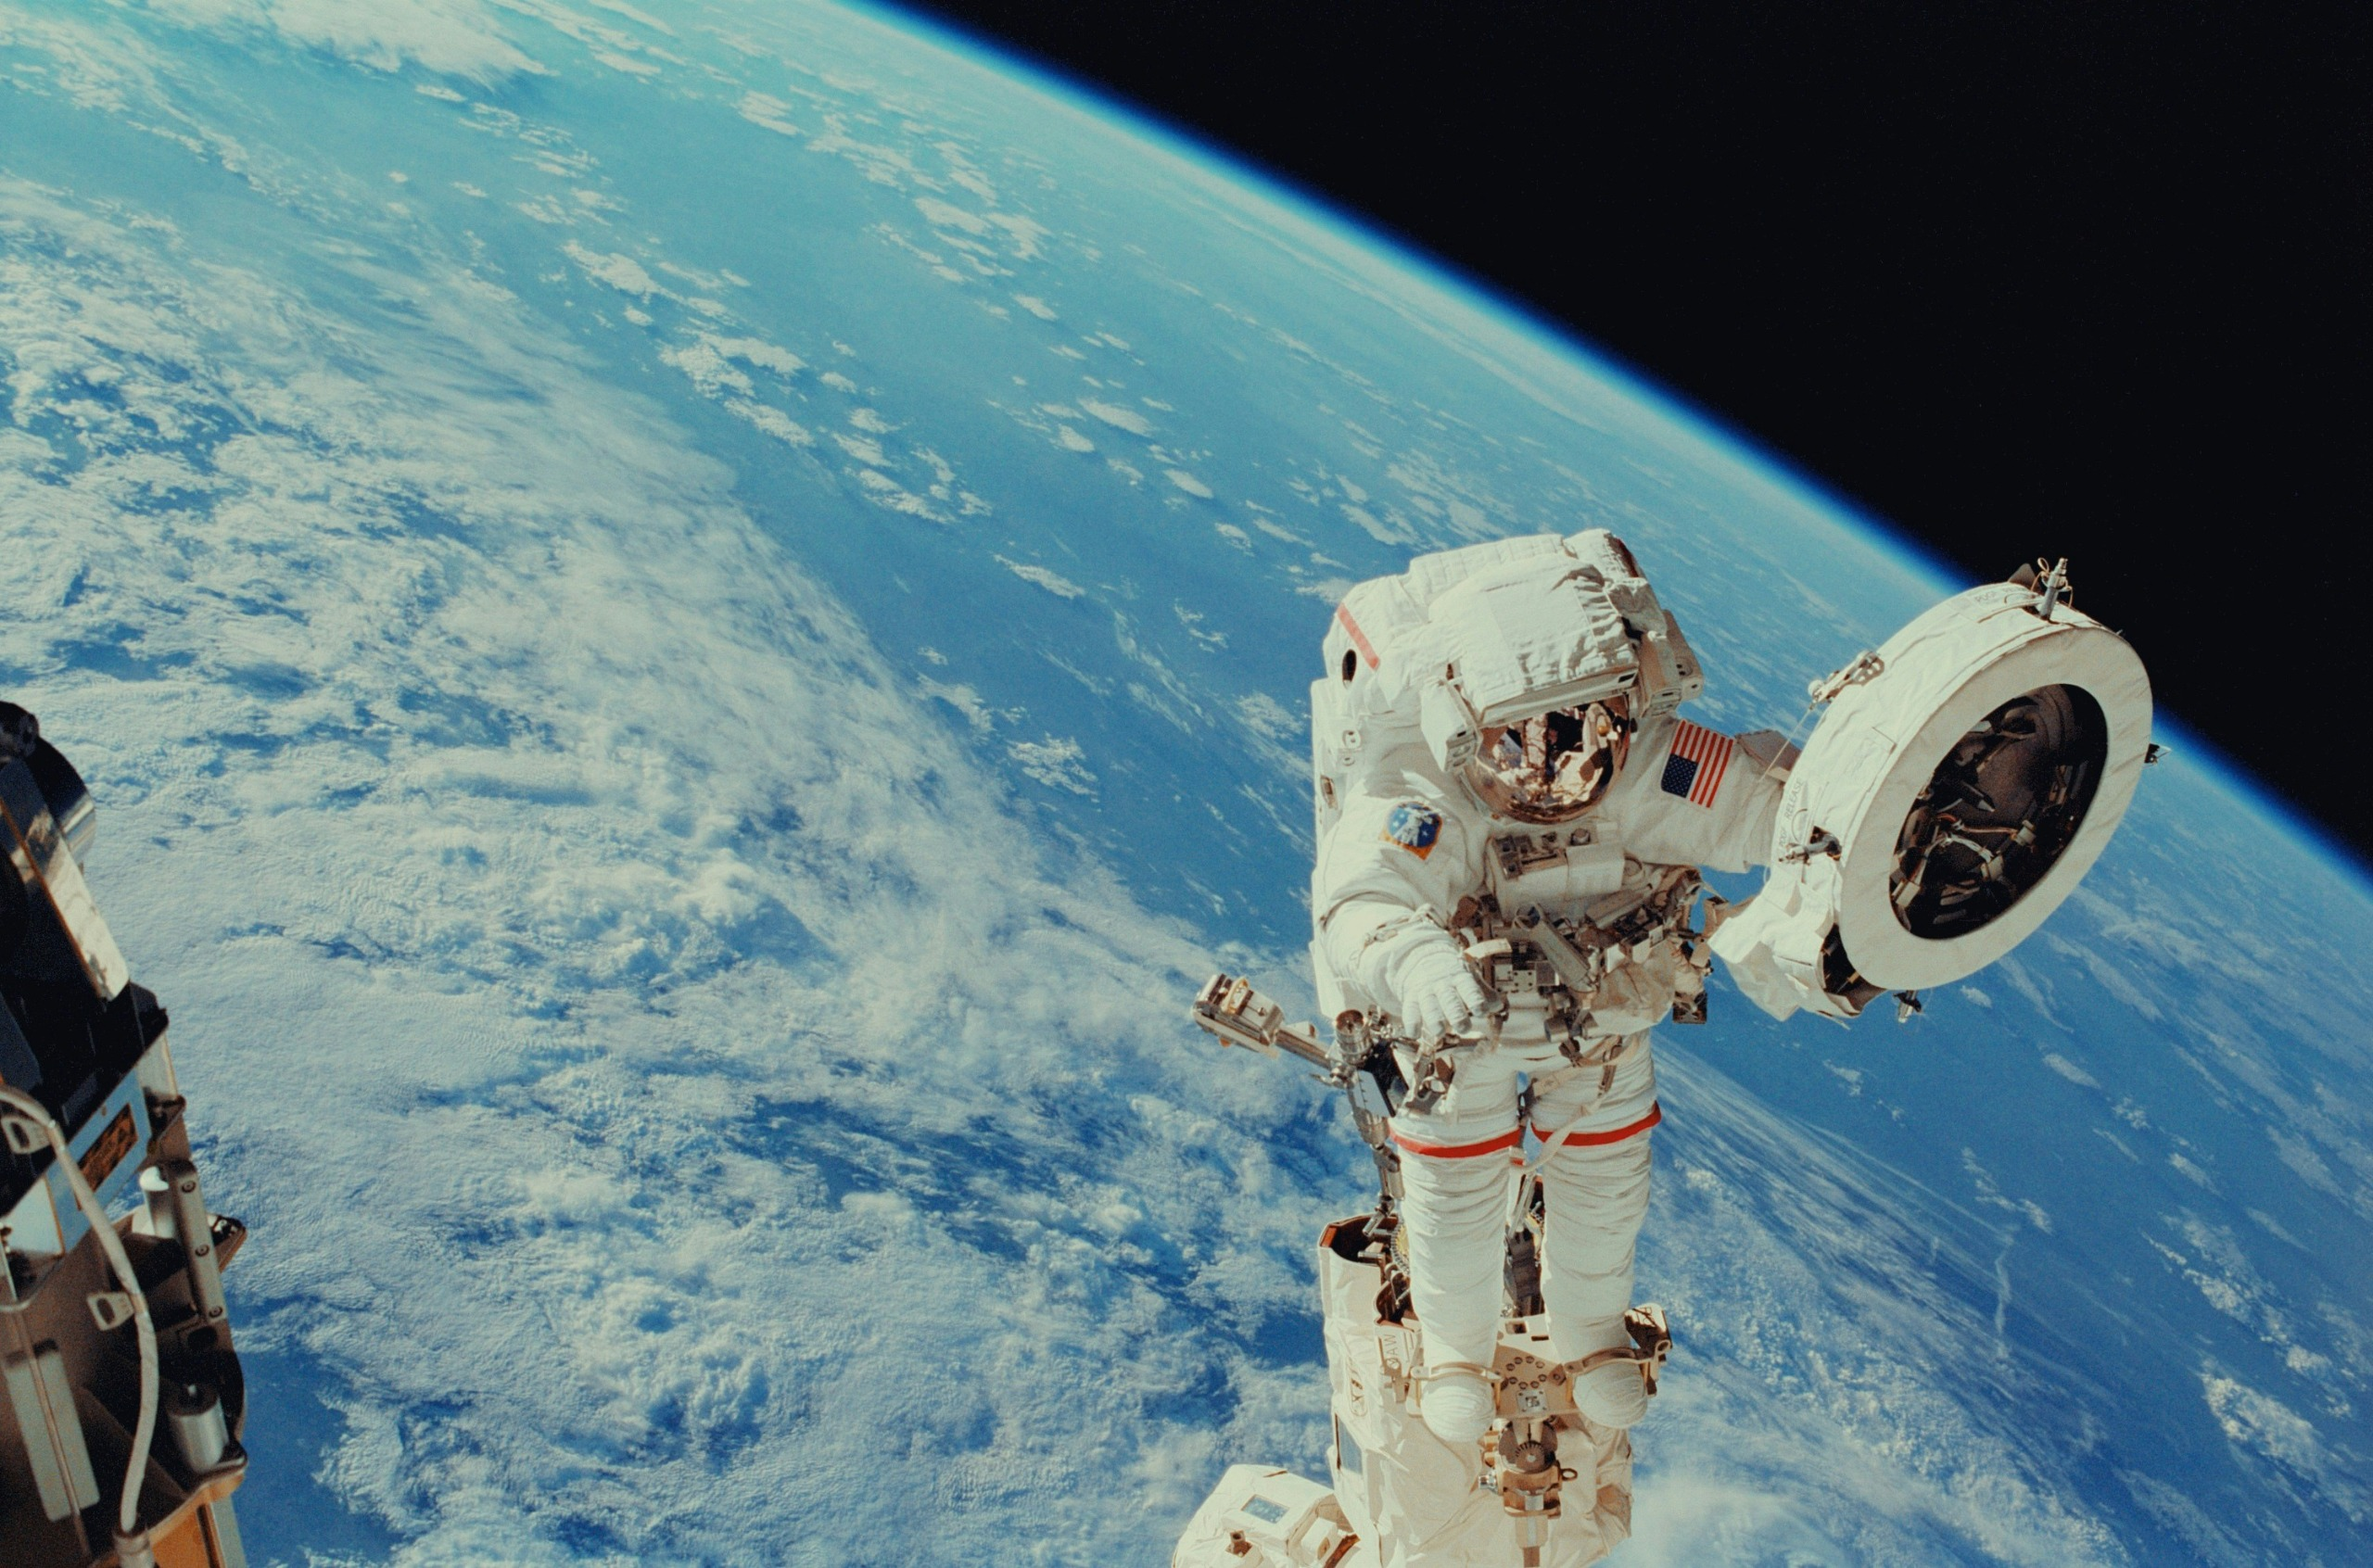
\includegraphics[height=157mm]{astrovital_portada.jpeg}};
\fill[navy,opacity=.40] (current page.north west) rectangle ([yshift=-157mm]current page.north east);
\fill[navy,opacity=.78] ([yshift=-105mm]current page.north west) rectangle ([yshift=-157mm]current page.north east);
\node[anchor=north west,text=white,font=\bfseries\large] at ([xshift=16mm,yshift=-14mm]current page.north west) {ASTROVITAL};
\node[anchor=north west,text=white,align=left,text width=178mm,font=\bfseries\fontsize{23}{27}\selectfont] at ([xshift=16mm,yshift=-112mm]current page.north west) {Connected health for\\safer missions};
\node[anchor=north west,text=white,align=left,text width=178mm,font=\small] at ([xshift=16mm,yshift=-138mm]current page.north west) {Health monitoring, analysis and follow-up in space.};
\end{scope}
\end{tikzpicture}%
}
\vspace*{149mm}
\heading{01  The challenge we address}{PURPOSE}
On long-duration missions, space radiation, changing gravity, isolation and distance from Earth call for greater autonomy in health monitoring. The challenge \textit{Create Health Monitoring Software for Astronauts on Space Missions} calls for visual tools to recognize changes and act on understandable information.
\begin{infobox}\textbf{Our response:} bring vital signs, history and interpretable alerts together in a platform offering scientific context and crew guidance as \textbf{support for monitoring and decisions}, without automatic clinical diagnosis.\end{infobox}
\heading{02  Value proposition}{WHY ASTROVITAL}
\par\noindent\begin{tabularx}{\linewidth}{@{}X@{\hspace{8mm}}X@{}}
\textbf{\color{blue}Measure} ECG, heart rate, SpO\textsubscript{2} and respiration from sensors. & \textbf{\color{blue}Understand} Reading freshness, charts and health trends.\\[6pt]
\textbf{\color{blue}Act} Interpretable alerts and guidance for verifying values. & \textbf{\color{blue}Contextualize} Station, orbit, Moon and Mars scenarios with NASA references.\\
\end{tabularx}
\vfill
{\scriptsize Official challenge: }\linktxt{View the challenge}{https://www.spaceappschallenge.org/2026/challenges/health-monitoring-software/}\par
{\scriptsize\color{muted}Cover photograph supplied by the team.}
\newpage
\heading{03  User experience}{ONE SYSTEM, SEVERAL MOMENTS}
\par\noindent\begin{tabularx}{\linewidth}{@{}>{\bfseries\color{blue}}p{13mm}>{\bfseries}p{40mm}X@{}}
01 & Sign in & Individual access to recent health readings and device status.\\[8pt]
02 & Connect sensors & ESP32 connection through Bluetooth Low Energy, telemetry reception and reading-validity checks.\\[8pt]
03 & Record information & Complement sensor readings with manual records, sleep, activity and wellbeing, according to available data.\\[8pt]
04 & Explore trends & Charts and history to compare measurements and changes over time.\\[8pt]
05 & Evaluate results & Rules incorporating signal quality, freshness, trends and the selected environment.\\[8pt]
06 & Review alerts & Understandable indications and suggested verification actions before continuing follow-up.\\
\end{tabularx}
\heading{04  Product modules}{FEATURES}
\par\noindent\begin{tabularx}{\linewidth}{@{}X@{\hspace{6mm}}X@{}}
\begin{infobox}\tinyhead{Health dashboard}\par\textbf{Indicators at a glance}\par Pulse, SpO\textsubscript{2} and respiration cards; current state, signal visualization and data freshness.\end{infobox}&
\begin{infobox}\tinyhead{Historical follow-up}\par\textbf{Visible changes}\par Time series, measurement history and trends for personal assessment.\end{infobox}\\[5pt]
\begin{infobox}\tinyhead{Capture environment}\par\textbf{Space context}\par Mission scenarios and physical and radiation references for understanding operating conditions.\end{infobox}&
\begin{infobox}\tinyhead{Alerts and assessment}\par\textbf{Explainable information}\par Transparent rules, attention messages and suggestions for reviewing sensors or results.\end{infobox}\\
\end{tabularx}
\heading{05  Design principles}{CLARITY IN DEMANDING MISSIONS}
The experience prioritizes visual hierarchy, quick reading, responsive navigation, Spanish and English interfaces, and a distinction between current and stale data. A missing result is not presented as zero: the interface communicates connection quality and signal availability.
\begin{navybox}{\color{white}\textbf{ASTROVITAL's central contribution}\par Physical capture + records + trends + decision rules + space context, brought together to support autonomous monitoring and risk communication.}\end{navybox}
\newpage
\heading{06  Technology architecture}{FROM SENSORS TO DECISIONS}
\begin{center}
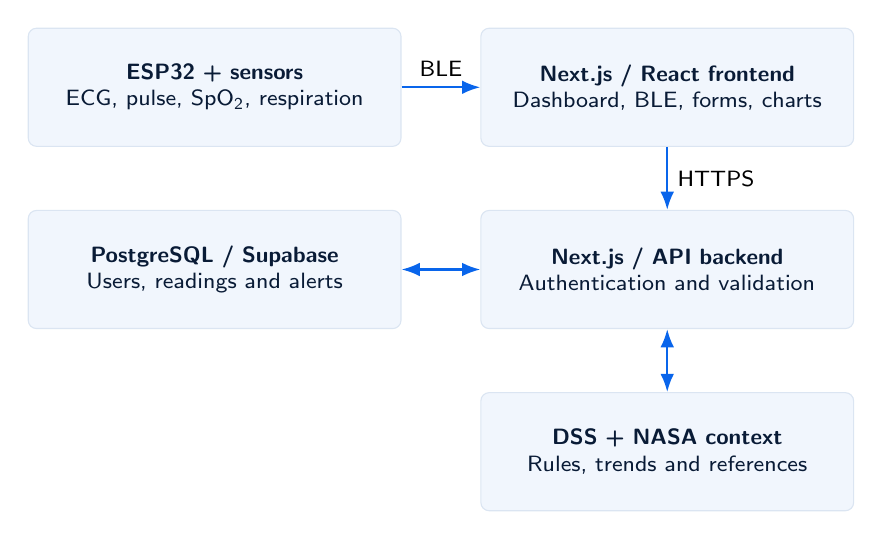
\begin{tikzpicture}[node distance=4.5mm,>=Latex,every node/.style={font=\footnotesize},mod/.style={draw=line,fill=light,rounded corners=3pt,text=navy,align=center,text width=45mm,minimum height=15mm},arr/.style={-Latex,thick,draw=blue}]
\node[mod] (a) {\textbf{ESP32 + sensors}\\ECG, pulse, SpO\textsubscript{2}, respiration};
\node[mod,right=10mm of a] (b) {\textbf{Next.js / React frontend}\\Dashboard, BLE, forms, charts};
\node[mod,below=8mm of b] (c) {\textbf{Next.js / API backend}\\Authentication and validation};
\node[mod,left=10mm of c] (d) {\textbf{PostgreSQL / Supabase}\\Users, readings and alerts};
\node[mod,below=8mm of c] (e) {\textbf{DSS + NASA context}\\Rules, trends and references};
\draw[arr] (a)--node[above]{BLE}(b);\draw[arr] (b)--node[right]{HTTPS}(c);\draw[arr,<->] (c)--(d);\draw[arr,<->] (c)--(e);
\end{tikzpicture}
\end{center}
\par\noindent\begin{tabularx}{\linewidth}{@{}>{\bfseries}p{40mm}X@{}}
Web interface & Independent Next.js, React and TypeScript frontend. Astronaut screens, history, device connection, manual records, environment and alerts.\\[7pt]
Backend services & REST API, sessions, validation, persistence and DSS at \texttt{GET /api/v1/me/dss}.\\[7pt]
Persistence & PostgreSQL in Supabase for profiles, readings, alerts and other application entities.\\[7pt]
Electronics & ESP32 firmware with sensors and BLE transport; local bridge tools and compatibility tests.\\[7pt]
Assessment engine & Decision tree with demonstration rules examining indicators, freshness, information quality, context and possible alerts.\\[7pt]
Deployment and quality & Separate frontend and backend services on Vercel; type checking, lint, builds, sensor tests and assessment tests.\\
\end{tabularx}
\heading{07  Technical flow}{TRACEABILITY}
\begin{infobox}\textbf{Capture} $\rightarrow$ \textbf{BLE reception or manual record} $\rightarrow$ \textbf{validation} $\rightarrow$ \textbf{storage} $\rightarrow$ \textbf{DSS analysis} $\rightarrow$ \textbf{visualization and alert}.\par
The DSS handles missing or stale readings and avoids conclusive assessments without sufficient information. Historical radiation references characterize the scenario; user vital signs come from the ESP32 or personal records.\end{infobox}
\heading{08  Evolution and potential}{VALUE FOR THE CHALLENGE}
The modular architecture separates capture, processing and presentation, supporting the progressive addition of physiological variables, sensors, environmental profiles and verification mechanisms without rebuilding the astronaut experience.
\newpage
\heading{09  NASA scientific data}{SPACE RADIATION REFERENCES}
The environmental module uses summaries of historical series attributed to \textbf{NASA Open Science Data Repository, RadLab}. They describe instrumental references from different missions and radiation context across scenarios.
\par\noindent\begin{tabularx}{\linewidth}{@{}>{\bfseries}p{31mm}p{59mm}>{\raggedleft\arraybackslash}p{23mm}X@{}}
\toprule Scenario & Mission / instrument & Records & Source\\\midrule
Mars surface & Curiosity · MSL-RAD & 274,998 & \linktxt{RadLab}{https://visualization.osdr.nasa.gov/radlab/gui/overview/}\\[5pt]
Lunar orbit & LRO · CRaTER-D1D2 & 71,626 & \linktxt{RadLab}{https://visualization.osdr.nasa.gov/radlab/gui/overview/}\\[5pt]
Space transit & Artemis I · Orion EAD-MU01 & 7,303 & \linktxt{RadLab}{https://visualization.osdr.nasa.gov/radlab/gui/overview/}\\\midrule
\multicolumn{2}{@{}l}{\textbf{Total reported historical observations}} & \textbf{353,927} & \linktxt{RadLab API}{https://visualization.osdr.nasa.gov/radlab/gui/data-api/}\\\bottomrule
\end{tabularx}
{\footnotesize\color{muted}Reported unit: $\mu\mathrm{Gy/h}$. Summaries are recorded in \texttt{data/radlab\_reference\_summaries.json}. These are instrumental references, not users' body doses. Counts and percentiles were supplied and have not been reproduced without the original CSV files.}
\heading{10  NASA sources for environmental context}{CATALOG AND REFERENCES}
\par\noindent\begin{tabularx}{\linewidth}{@{}>{\bfseries}p{43mm}X@{}}
NASA Earthdata & \linktxt{Earthdata Search}{https://search.earthdata.nasa.gov/}: Earth observation data discovery portal.\\[6pt]
Landsat & \linktxt{NASA Landsat}{https://landsat.gsfc.nasa.gov/}: Earth observation program and mission documentation.\\[6pt]
Perseverance / MEDA & \linktxt{NASA PDS atmospheric archive}{https://pdsatmospheres.nmsu.edu/data_and_services/atmospheres_data/PERSEVERANCE/meda.html}: Martian weather conditions.\\[6pt]
LRO / Diviner & \linktxt{NASA PDS Diviner}{https://pds-geosciences.wustl.edu/missions/lro/diviner.htm}: lunar thermal references.\\[6pt]
NASA Human Research Program & \linktxt{Five Hazards of Human Spaceflight}{https://www.nasa.gov/hrp/hazards/}: human exploration risk factors.\\[6pt]
NASA-STD-3001 & \linktxt{Human-System Standard, Vol. 2}{https://www.nasa.gov/reference/nasa-std-3001v2/}: human health and spaceflight requirements.\\[6pt]
NASA HRP evidence & \linktxt{Sleep report}{https://humanresearchroadmap.nasa.gov/Evidence/reports/Sleep.pdf} and \linktxt{risk repository}{https://humanresearchroadmap.nasa.gov/}: conceptual support for indicators and risks.\\
\end{tabularx}
\begin{infobox}\textbf{How these sources are used.} RadLab supplies the DSS's historical quantitative radiation reference. MEDA, Diviner and HRP are documentary scientific references. Earthdata and Landsat are related NASA discovery portals; no unproven operational integration is claimed.\end{infobox}
\heading{11  Interpretation and reliability}{EXPLAINABLE ANALYSIS}
The decision tree combines signal availability, reference ranges, reading changes and mission context. It distinguishes current, historical and invalid data and communicates observations in understandable language. The scope is \textbf{monitoring and guidance}, not diagnosis or flight medical validation.
\newpage
\heading{12  Artificial intelligence disclosure}{PROCESS TRANSPARENCY}
Generative artificial intelligence, \textbf{OpenAI's ChatGPT and Codex}, assisted ASTROVITAL throughout development, including \textbf{code generation}. Support covered technical work, research and communication, with integration and final decisions by the team. The AstroVital SVG logo was created with AI assistance.
\par\noindent\begin{tabularx}{\linewidth}{@{}>{\bfseries}p{48mm}X@{}}
Programming and code generation & Drafts and reviews of React components, TypeScript/JavaScript logic, backend services, interfaces, data structures and integration functions.\\[10pt]
Software architecture & Support defining layers, ESP32-BLE-frontend communication, API routes, storage and separation of responsibilities.\\[10pt]
DSS model and analysis & Decision-rule design and improvements, signal interpretation, state handling and risk explanations.\\[10pt]
Debugging and verification & Failure analysis, proposed fixes, test cases, telemetry reasoning and consistency reviews.\\[10pt]
Interface and experience & Visual layout, indicator hierarchy, alert messages, microcopy and interaction proposals.\\[10pt]
Scientific documentation & NASA source organization, documentation synthesis, technical rationale and project materials.\\
\end{tabularx}
\begin{navybox}{\color{white}\textbf{Team responsibility.} AI supported design, programming, testing and documentation. The developers integrated and adapted ASTROVITAL as a prototype and own the engineering decisions, code review and presentation of results.}\end{navybox}
\heading{13  Project vision}{TECHNOLOGY SERVING THE CREW}
ASTROVITAL proposes an accessible way to observe astronaut health, connect personal data with complex space environments and turn information into understandable alerts. The experience seeks to strengthen crew self-care and preparedness for increasingly long missions.
\vfill
{\color{blue}\rule{\linewidth}{1pt}}\par
\textbf{ASTROVITAL}\hfill{\footnotesize\color{muted}Project brief · 2026}
\newpage
\heading{14  Direct access to resources and datasets}{FULL CLICKABLE LINKS}
The following links provide direct access to ASTROVITAL, its public repository and the scientific references consulted. Full addresses are displayed for verification and browser access.
\begin{infobox}
\tinyhead{Product and source code}\par\textbf{Deployed platform}\par\url{https://astrovital-health.vercel.app/login}\par\vspace{3pt}
\textbf{ASTROVITAL repository}\par\url{https://github.com/AMVMesias/ASTROVITAL}\par\vspace{3pt}
\textbf{MIT license in the repository root}\par\url{https://github.com/AMVMesias/ASTROVITAL/blob/main/LICENSE}\par\vspace{3pt}
\textbf{Official project challenge}\par\url{https://www.spaceappschallenge.org/2026/challenges/health-monitoring-software/}
\end{infobox}
\heading{15  NASA OSDR RadLab}{HISTORICAL RADIATION SERIES}
\textbf{Primary source of the three series included in the DSS:} NASA Open Science Data Repository, RadLab. MSL-RAD (Curiosity), CRaTER (LRO) and EAD-MU01 (Orion / Artemis I) are documented through the same portal; undocumented filtered download links are not claimed.
\par\noindent\begin{tabularx}{\linewidth}{@{}>{\raggedright\arraybackslash\bfseries\color{navy}}p{39mm}X@{}}
Official RadLab portal & \url{https://visualization.osdr.nasa.gov/radlab/gui/overview/}\\[6pt]
Charts and time series & \url{https://visualization.osdr.nasa.gov/radlab/gui/time-series-plots/}\\[6pt]
API documentation & \url{https://visualization.osdr.nasa.gov/radlab/gui/data-api/}\\
\end{tabularx}
\heading{16  Other NASA sources}{SCIENTIFIC ARCHIVES AND PORTALS}
\par\noindent\begin{tabularx}{\linewidth}{@{}>{\raggedright\arraybackslash\bfseries\color{navy}}p{40mm}X@{}}
MEDA / Perseverance & \url{https://pdsatmospheres.nmsu.edu/data_and_services/atmospheres_data/PERSEVERANCE/meda.html}\\[6pt]
DOI MEDA & \url{https://doi.org/10.17189/1522849}\\[6pt]
NASA Earthdata Search & \url{https://search.earthdata.nasa.gov/}\\[6pt]
NASA Landsat & \url{https://landsat.gsfc.nasa.gov/}\\[6pt]
LRO / Diviner & \url{https://pds-geosciences.wustl.edu/missions/lro/diviner.htm}\\
\end{tabularx}
\vfill
{\footnotesize\color{muted}RadLab links lead to the official service and its time-series explorer. The exact historical file filter selections are not included in this document.}
\newpage
\heading{17  NASA space health reports}{COMPLETE REFERENCES}
These official sources support discussion of cardiovascular risks, decompression, extravehicular injuries, physical capacity and sleep. The full URLs are clickable.
\renewcommand{\arraystretch}{1.13}
\begin{infobox}
\tinyhead{Reference health standard}\par
\textbf{NASA-STD-3001, Volume 2}\par
\url{https://www.nasa.gov/reference/nasa-std-3001v2/}
\end{infobox}
\vspace{3pt}
{\small\bfseries\color{navy}Cardiovascular risks}\par
{\footnotesize\url{https://humanresearchroadmap.nasa.gov/Evidence/reports/Cardio%20Risk%20EB%202022%20FINAL_4-3-2023.pdf}}\par\vspace{6pt}
{\small\bfseries\color{navy}Extravehicular activity (EVA) injuries}\par
{\footnotesize\url{https://humanresearchroadmap.nasa.gov/Evidence/other/EVA%20Injury%20Evidence%20Report%20FINAL_6-14-2023.pdf}}\par\vspace{6pt}
{\small\bfseries\color{navy}Hypoxia and decompression sickness}\par
{\footnotesize\url{https://humanresearchroadmap.nasa.gov/Evidence/other/Evidence%20Report%20Hypoxia%20and%20DCS_FINAL_1-8-2024.pdf}}\par\vspace{6pt}
{\small\bfseries\color{navy}Aerobic and muscular capacity}\par
{\footnotesize\url{https://humanresearchroadmap.nasa.gov/Evidence/reports/Evidence%20report%20aerobic%20and%20muscle_FINAL%204-3-2024.pdf}}\par\vspace{6pt}
{\small\bfseries\color{navy}Sleep loss and sleep disturbances}\par
{\footnotesize\url{https://humanresearchroadmap.nasa.gov/Evidence/reports/Sleep.pdf}}\par\vspace{6pt}
{\small\bfseries\color{navy}General medical risks - NASA Human Research Roadmap}\par
{\footnotesize\url{https://humanresearchroadmap.nasa.gov/Risks/print/?i=95}}\par
\vfill
\begin{navybox}
{\color{white}\bfseries ASTROVITAL: connected health for safer missions}\par
{\color{white}A monitoring system bringing biometric signals, historical indicators and space knowledge into an understandable crew experience.}
\end{navybox}

\newpage
\heading{18  Image credits}{PHOTOGRAPHS AND SOURCES}
The project uses photographs published by NASA on Unsplash. The individual source pages and the contributor profile are linked below.
\begin{infobox}
\textbf{NASA profile on Unsplash}\par
\url{https://unsplash.com/es/@nasa}\par
\end{infobox}
\vspace{5pt}
{\small\bfseries\color{navy}Earth and satellite view}\par
\href{https://unsplash.com/es/fotos/vista-de-la-tierra-y-satelite-yZygONrUBe8}{\textcolor{blue}{\nolinkurl{https://unsplash.com/photos/yZygONrUBe8}}}\par
\vspace{5pt}
{\small\bfseries\color{navy}Soyuz rocket launch}\par
\href{https://unsplash.com/es/fotos/el-cohete-soyuz-se-lanza-desde-la-plataforma-de-lanzamiento-de-baikonur-JkaKy_77wF8}{\textcolor{blue}{\nolinkurl{https://unsplash.com/photos/JkaKy_77wF8}}}\par
\vspace{5pt}
{\small\bfseries\color{navy}Astronaut beside a satellite}\par
\href{https://unsplash.com/es/fotos/fotografia-de-un-astronauta-junto-al-satelite-OLlj17tUZnU}{\textcolor{blue}{\nolinkurl{https://unsplash.com/photos/OLlj17tUZnU}}}\par
\vspace{5pt}
{\small\bfseries\color{navy}Astronaut on the Moon beside the flag}\par
\href{https://unsplash.com/es/fotos/astronauta-de-pie-en-la-luna-junto-a-la-bandera-de-eeuu-U2uKrI4lci8}{\textcolor{blue}{\nolinkurl{https://unsplash.com/photos/U2uKrI4lci8}}}\par
\vspace{5pt}
{\small\bfseries\color{navy}Extravehicular activity}\par
\href{https://unsplash.com/es/fotos/astronauta-de-la-nasa-realiza-actividad-extravehicular-gYwfpVI2JzM}{\textcolor{blue}{\nolinkurl{https://unsplash.com/photos/gYwfpVI2JzM}}}\par
\vspace{8pt}
\textbf{Unsplash License:} \url{https://unsplash.com/license}

\end{document}
